\chapter{Vorbetrachtungen}

Im folgenden werden die verwendeten Technologien betrachtet. Als Versionsverwaltungssoftware wurde Git\cite{git} auf der Platform Github\cite{github} verwendet, worauf nicht weiter eingegangen wird. Zum Erstellen der Simulation wurde Omnet++\cite{omnet} mithilfe des MiXiM-Frameworks\cite{mixim} benutzt.

\section{Evaluation von Systemen}

Im Entwicklungsprozess eines jeden Systems müssen neue Teile oder Module evaluiert werden. Für das Testen gibt es verschiedene Möglichkeiten, die einem zur Verfügung stehen. Im frühen Stadium der Entwicklung bietet das Abschätzen von gewissen Parametern eine kostengünstige Variante zum Bestimmen von Designparametern. Das kann noch vor einer ersten Implementierung und daher auch ohne Messungen durchgeführt werden. Allerdings sind diese Ergebnisse oftmals sehr grob und es lässt sich auch nicht jeder Wert so einfach bestimmen. \newline
Es ist daher notwendig genauere Tests durchzuführen. Wenn man ein komplett implementiertes und produziertes System anschließend testen möchte kann das sehr teuer werden, sollten viele Fehler auftreten oder schlimmer, wenn man zum Beispiel merkt, dass das gewählt Modell das gewünschte Ziel nicht befriedigend erfüllen kann und daher viel bisherige Arbeit verworfen werden müsste. \newline
Man kann diesen Problemen zuvor kommen, indem man noch vor der ersten Implementierung eines Systems Simulationen und Emulationen erstellt und Prototypen anfertigt. Das senkt die Kosten mitunter erheblich und es lassen sich beinahe alle Parameter des zukünftigen Produkts überprüfen, auch wenn es das Testen des fertigen Produkts nicht komplett ersetzen kann.

\paragraph{Simulation}

Eine Simulation ist ein Modell eines Systems, welches dieses passend abbildet. Mit diesem Modell kann herausgefunden werden, was im realen System später umsetzbar ist. Der Zustand eines solchen Modells ändert sich im Laufe der (Simulations-)Zeit. Daher führt das Modell Zustandsübergange durch, welche als Events bezeichnet werden. Man kann Systeme nach den Zeitpunkten an denen Zustandswechsel möglich sind, in analoge und diskrete unterteilen. Wie der Name vermuten lässt können im analogen Fall zu jeder Zeit Zustandsübergänge stattfinden, im diskreten dagegen nur zu bestimmten Zeitpunkten.\\
Eine Simulation eignet sich zu jedem Zeitpunkt des Produktentwurfs sehr gut. Große Vorteile sind, dass auf diese Weise schon sehr früh getestet werden kann und sich Simulationen sehr kostengünstig erstellen lassen, da keine besondere Hardware notwendig ist.

\paragraph{Emulationen}

Eine Emulation ist die Implementierung eines Systems, welche den kompletten Funktionsumfang des Entwurfs abdeckt. Diese kann mit einer Hardwarebeschreibungssprache wie VHDL definiert werden und auf einem FPGA oder innerhalb eines Netzwerks von FPGAs ausgeführt werden. Man spricht daher von einer homogenen Hardwareplattform.

\paragraph{(Rapid) Prototyping}

Ein Prototyp ist ebenfalls eine Implementierung eines Systems, die den kompletten Funktionsumfang des Entwurfs abdeckt, allerdings geringere Anforderungen and Timing, Größe und Kosten stellt. Prototypen sind zum Beispiel oftmals wesentlich größer als das Endprodukt. Wenn er alle sonstigen Anforderungen zur Genüge erfüllt, so kann er in das finale Design umgewandelt werden und verliert bei diesem Prozess alle Grenzen des Prototyps. Im Gegensatz zur Emulation kommt eine heterogene Hardwareplattform zum Einsatz. So können etwa fertige Prozessoren, Speicher, weiterhin FPGAs oder spezielle Chips wie ein ASIC zum Einsatz kommen.

\endgraf

Für die Arbeit ist die Entscheidung auf eine Simulation gefallen. Man kann sich dabei auf die wesentlichen Funktionen konzentrieren und grundsätzliche Überlegungen über die genaue Umsetzung von gewissen Bauteilen zunächst außer Acht lassen. So ist die genaue Implementierung der einzelnen Komponenten des Sensors für diese Arbeit beispielsweise nicht so relevant, da eher das gesamte Verhalten der Sensorknoten und deren Energiemanagement von Bedeutung sind. Ein Modell muss stets nur so genau spezifiziert werden wie nötig und so gut wie nie mit der Komplexität der Realität übereinstimmen. \newline
Der Fokus der Arbeit liegt daher auch auf dem Verwalten von Umweltparametern, der Erfassung dieser durch Sensoren auf vielen verschiedenen Sensorknoten. Wie genau die einzelnen Bauteile technisch aufgebaut sind ist für die theoretische Betrachtung natürlich von Bedeutung, soll jedoch nicht bis ins kleinste Detail simuliert werden.

\section{Sensoren}

Den Hauptgegenstand in der Simulation bilden Sensoren, welche auf Sensorknoten angebracht sind. Ein solcher Knoten kann dann wiederum ein oder mehrere Sensoren besitzen.\newline
Sensoren sind das technische Gegenstück zu den menschlichen Sinnen, denn sie können physikalische oder chemische Eigenschaften wahrnehmen. Dabei arbeiten Sensoren allerdings noch wesentlich genauer, denn es lassen sich Messgrößen quantitativ exakt bestimmen.\newline

\begin{figure}[htbp]
\centering
\caption{Abstraktes Sensor Modell}
\label{fig:AbstraktesSensorModell}
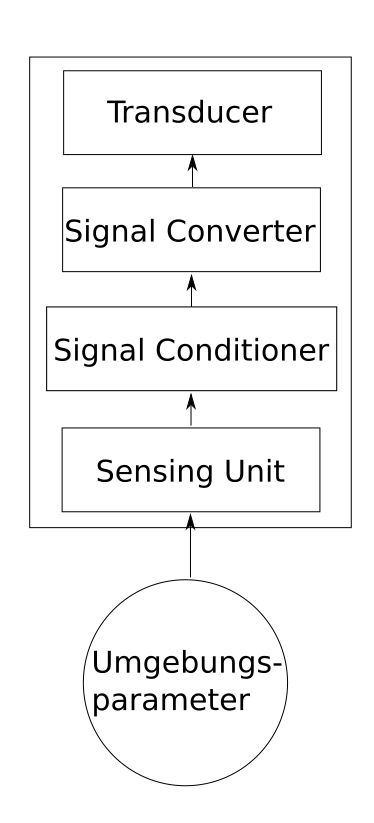
\includegraphics[height=0.7\textheight]{AbstraktesSensorModell}
\end{figure}

Allgemein ist ein Sensor wie in Abbildung \ref{fig:AbstraktesSensorModell} aufgebaut. Die SensingUnit, zu deutsch Aufnehmer, ist dabei das Herzstück, denn es ist das Bauteil, in dem der gesuchte Wert aus der Umgebung aufgenommen wird. Je nach Sensor ist dieser Wert jedoch nicht direkt interpretierbar. Das Signal wird daher zunächst aufbereitet. Zum einen kann das bedeuten, falls der Messimpuls nur sehr kurz war, diesen zu verlängern, sodass folgende Bauteile verwertbare Eingaben bekommen können. Zum anderen kann es nötig sein, dass ein analoges in ein digitales Signal umgewandelt werden muss. Diese Aufgaben werden durch Signalformer und Signalwandler übernommen.\newline
Zuletzt muss das Signal noch durch einen Messumformer aus einem bloßen digitalen Wert ohne direkte Bedeutung in einen Messwert in der benötigten Messeinheit umgewandelt werden. Dieser Wert kann dann über eine Schnittstelle nach außen gegeben werden und von anderen Teilen auf einem Sensorknoten verarbeitet werden.

\subsection{Beispiele für Sensoren}

Im folgenden Abschnitt werden ein paar verschiedene Beispiele für Sensoren vorgestellt. Es wird für die in der Implementierung umgesetzten Sensoren für Temperatur, Helligkeit, Luftdruck und Luftfeuchtigkeit jeweils ein Beispiel erläutert.

\paragraph{Temperatur}

Vermutlich bedingt durch die große Verbreitung und die bereits lange Existenz von Temperaturfühlern gibt es eine sehr hohe Zahl verschiedener Möglichkeiten Temperatur zu messen, wobei sich die verschiedenen Umsetzung zum Teil auch sehr stark unterscheiden. Dabei gibt es sowohl Sensoren mit passiven, als auch mit aktiven Aufnehmern.\newline
Ein Beispiel für eine Umsetzung ist ein Temperatursensor mit Aufnehmer in Form eines Heißleiters. Dieser verringert seinen Widerstand, wenn seine Temperatur steigt. Es kann nun eine stets konstante Spannung an den Heißleiter angelegt werden, um auf die Temperatur des Bauteils zu schließen. Da zum abgreifen der Messwerte eine Spannung von außen angelegt werden muss, liegt ein passiver Aufnehmer vor.

\begin{figure}[htbp]
\centering
\caption{Deutschlandkarte der mittleren Temperatur zwischen 1961 und 1990}
\label{fig:temperatur}
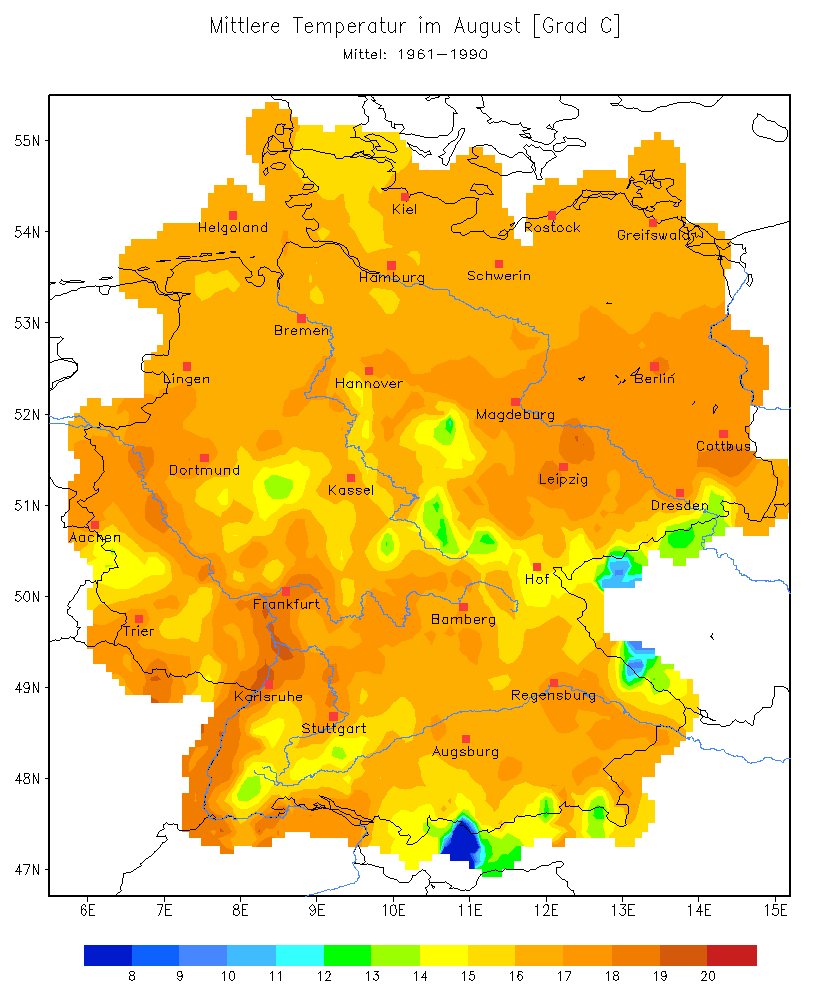
\includegraphics[width=\textwidth]{temperatur}
\end{figure}

\paragraph{Helligkeit}

Ein Lichtsensor oder auch Photodetektor dient dazu, um die stärke des einfallenden Lichts zu bestimmen, also die Helligkeit. Diese können unter Nutzung des photoelektrischen Effekts ganz ähnlich zum vorgestellten Temperatursensor mit Heißleiter genutzt werden. Die sogenannte Photoleitung bezeichnet hierbei die Zunahme der Leitfähigkeit, durch steigende Bestrahlung. Um den Sensor mit einem aktiven Aufnehmer zu nutzen, kann ein Sensor auch mit dem photovoltaische Effekt gebaut werden. Dieser wird ebenfalls bei der Gewinnung von elektrischer Energie durch das Sonnenlicht benutzt. Je stärker die einfallende Sonnenenergie auf der Photovoltaikfläche ist, um so mehr Energie wird erzeugt und um so größer ist die Helligkeit.

\paragraph{Luftdruck}

Auch von Drucksensoren gibt es sehr viele verschiedene Arten, welche auf unterschiedliche Weise funktionieren. Dabei gibt es Sensoren, welche lediglich Messwertänderungen feststellen können und andere, die wiederum auch statische Werte ermitteln können. Ein Beispiel für die zweite Variante ist ein piezoresistiver Drucksensor. Bei diesem befindet sich im Aufnehmer eine Membran, deren Position sich durch unterschiedlich hohen Druck verändert. Um diese Bewegung nun messbar zu machen, werden auf der Membran Widerstände aufgebracht.

\paragraph{Luftfeuchtigkeit}

Sensoren zur Bestimmung der Luftfeuchtigkeit werden auch Hygrometer genannt. Eine Variante dieser ist ein Absorptionshygrometer. Dabei befindet sich eine Schicht zwischen 2 Elektroden, welche die Feuchtigkeit der Umgebung gut aufnehmen kann. Diese Schicht wird als hygroskopische Schicht bezeichnet. Wenn nun eine Spannung angelegt wird, dann ist der Widerstand dieser Schicht abhängig von der Feuchtigkeit und somit kann wiederum indirekt auf diese geschlossen werden.

\begin{figure}[htbp]
\centering
\caption{Deutschlandkarte: Beispielverteilung der Luftfeuchtigkeit}
\label{fig:feuchtigkeit}
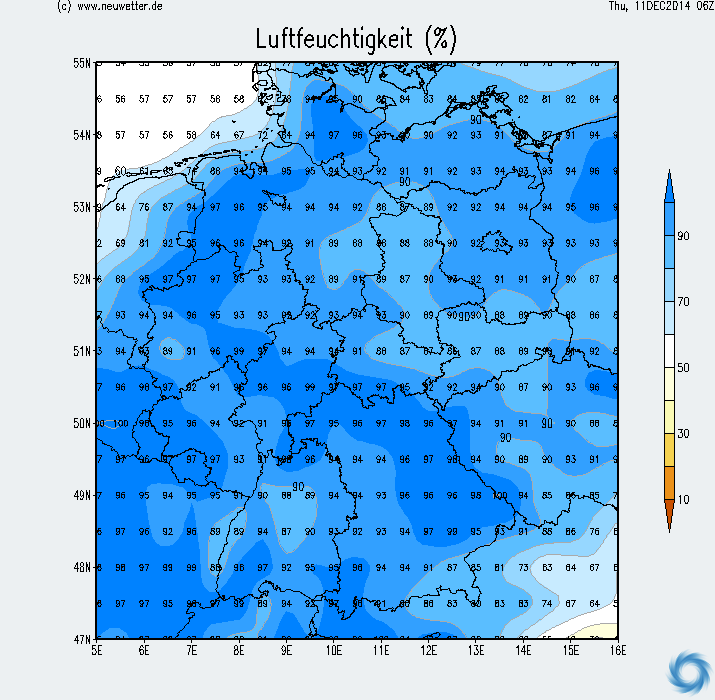
\includegraphics[width=\textwidth]{feuchtigkeit}
\end{figure}

\section{Sensorknoten}

Sensorknoten gibt es natürlich in verschiedenen Formen und Größen, doch gewisse Grundelemente sind in jedem Sensorknoten gleich. In Abbildung \ref{fig:sensornode} ist ein grober Aufbau beschrieben. In der heutigen Zeit befinden sich dabei alle Bauteile auf einem einzigen Chip, man spricht daher von einem System-on-a-Chip.\newline
Natürlich ist das wohl charakteristischste Bauteil, denn es macht einen Netzwerkknoten zum Sensorknoten, ein Sensor. Es ist ebenso möglich, dass ein Sensorknoten viele verschiedene Sensoren besitzt, um an der Position mehrere verschiedene Parameter aufnehmen zu können.\newline
Um aber mit den Messwerten etwas anfangen zu können, sind auch andere Bauteile essentiell. 

\begin{itemize}
\item Ein Prozessor, typischer Weise auf einem Mikrocontroller, muss sich dabei um die Steuerung der anderen Bauteile kümmern.
\item Ein Funkmodul ermöglicht dem Knoten die Kommunikation mit Anderen in seiner erreichbaren Umgebung. Nur dadurch ist es möglich in großflächigen Netzwerken die Daten auswerten zu können, da es in manchen Gebieten sogar unmöglich sein kann, die Knoten nach dem verstreuen noch direkt zu erreichen.
\item Ein Speicher sollte ebenfalls auf einem Knoten vorhanden sein. Zum einen müssen natürlich Programme, die der Prozessor ausführt gespeichert werden. Ebenso ist es denkbar, dass die Funkkommunikation gelegentlich für längere Zeit abgeschaltet wird, um so Energie zu sparen. Wenn innerhalb dieses Zeitraums relevante Messwerte bestimmt wurden, so sollen diese natürlich nicht einfach verfallen, sondern bis zur nächsten Funkverbindung gesichert werden.
\item Irgend eine Art von Energiequelle ist auch für einen Sensorknoten entscheidend, um funktionieren zu können. Dazu gehört typischer Weise eine Batterie. Weiterhin ist es denkbar, durch energy harvesting zusätzlich Energie zu gewinnen. Da dies aber nicht unbedingt rund um die Uhr möglich ist, muss auch in diesem Fall die gewonnene Energie zunächst gespeichert werden.
\end{itemize}

\begin{figure}[htbp]
\centering
\caption{Abstraktes Sensornoten Modell}
\label{fig:sensornode}
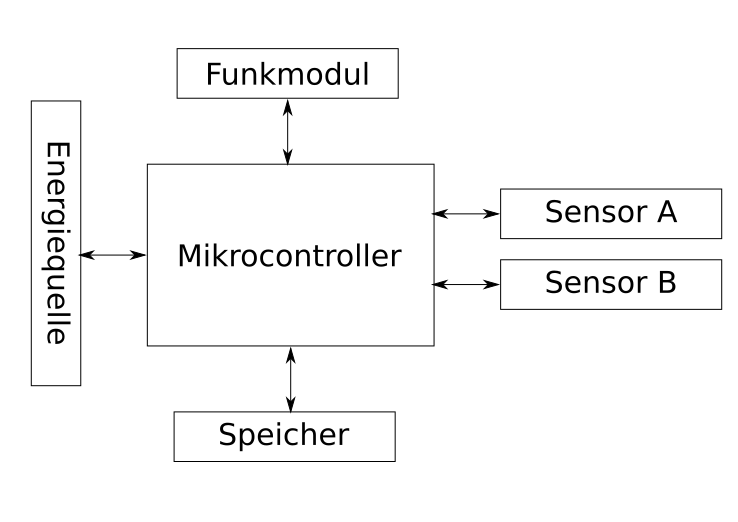
\includegraphics[width=\textwidth]{AbstraktesSensorknotenModell}
\end{figure}

\section{Sensornetzwerke}

Da ein einzelner Sensorknoten nur sehr begrenzt einsetzbar ist, werden die immer kleiner und mobiler werdenden Knoten oft zu großen Netzwerken verbunden. Dadurch ist es möglich große Flächen mit den Messwerkzeugen abzudecken. So ist es möglich detaillierte Daten von einem Gebieten zu erhalten.\newline
Bei einem sehr großen Netzwerk ist ein gutes Routing sehr wichtig, besonders da die Knoten sehr abhängig von der effizienten Nutzung der Energiequelle sind. Für das Übertragungsprotokoll kommt dabei meist der Standard IEEE 802.15.4 zum Einsatz, da dieser für Drahtlose Kommunikation mit niedriger Übertragungsrate und für Geräte mit geringer Leistungsaufnahme ausgelegt ist. Es deckt lediglich die unteren beiden Schichten des OSI-Modells ab.\newline
Die Verbindung zu Anwendungsschicht stellt dann beispielsweise das ZigBee-Framework dar. 